\documentclass[en,black,normal,10pt]{elegantnote}
\usepackage{colortbl} % Required for colored rows
\usepackage{xcolor}
\usepackage{lipsum} % Required for generating dummy text
\usepackage{tikz}
\usepackage{caption}
\usetikzlibrary{positioning}

\setlength{\parindent}{0pt}

\title{DSAA 5002 - HW1}

%\version{Fall Semester 2023}

\author{50015976 Ruiming ZHANG}
%\institute{Elegant\LaTeX{} Program}

\date{}

\usetikzlibrary{shapes,arrows}

\begin{document}

\maketitle
% logo
%\centerline{\includegraphics[width=0.2\textwidth]{logo-blue}}

\section*{Q1 [15 Marks]}

Given the transaction database below,set the minimum support count to 2 and the minimum confidence level to 60\% to find the strong association rule.
Generate the set $C_3$ of the candidate 3-itemset, using prunning on Apriori principle.

\definecolor{Gray}{gray}{0.85} % Define a custom color

\subsection*{Solution:}

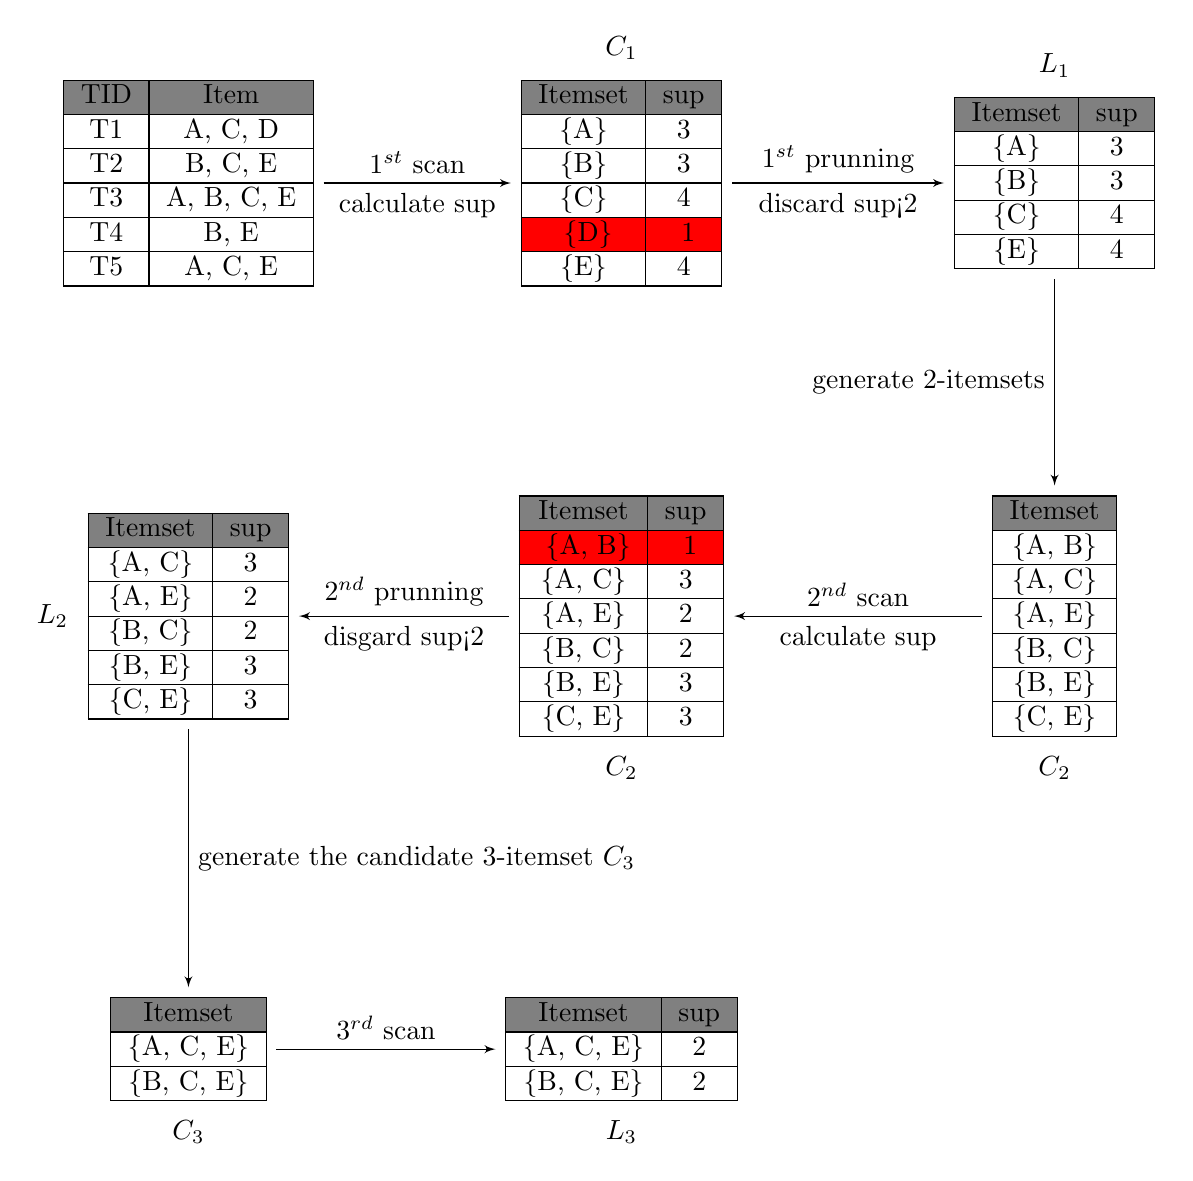
\begin{tikzpicture}[node distance = 5.5cm, auto]
    % Define block styles
    \tikzstyle{block} = [rectangle, fill=none,
                        text centered, rounded corners, minimum height=4em]
    \tikzstyle{line} = [draw, -latex']

    % Place nodes
    \node [block] (item1) {
      \begin{tabular}{|c|c|c|}
        \hline
          \rowcolor{Gray} % Set the color of the first row to gray
          TID & Item \\
          \hline
          T1 & A, C, D \\
          \hline
          T2 & B, C, E \\
          \hline
          T3 & A, B, C, E \\
          \hline
          T4 & B, E \\
          \hline
          T5 & A, C, E \\
          \hline
      \end{tabular}
    };

    \node [block, right  of=item1, label=above:$C_1$] (scan1) {
      \begin{tabular}{|c|c|c|}
        \hline
        \rowcolor{Gray} % Set the color of the first row to gray
        Itemset & sup \\
        \hline
        {\{A\}} & 3 \\
        \hline
        {\{B\}} & 3 \\
        \hline
        {\{C\}} & 4 \\
        \hline
        \cellcolor{red} {\{D\}} & \cellcolor{red} 1 \\
        \hline
        {\{E\}} & 4 \\
        \hline
      \end{tabular}
    };

    \node [block, right of=scan1, label=above:$L_1$] (prunning1) {
      \begin{tabular}{|c|c|c|}
        \hline
        \rowcolor{Gray} % Set the color of the first row to gray
        Itemset & sup \\
        \hline
        {\{A\}} & 3 \\
        \hline
        {\{B\}} & 3 \\
        \hline
        {\{C\}} & 4 \\
        \hline
        {\{E\}} & 4 \\
        \hline
      \end{tabular}
    };

    \node [block, below of=prunning1, label=below:$C_2$] (item2) {
      \begin{tabular}{|c|c|}
        \hline
        \rowcolor{Gray} % Set the color of the first row to gray
        Itemset \\
        \hline
        {\{A, B\}} \\
        \hline
        {\{A, C\}} \\
        \hline
        {\{A, E\}} \\
        \hline
        {\{B, C\}} \\
        \hline
        {\{B, E\}} \\
        \hline
        {\{C, E\}} \\
        \hline 
      \end{tabular}
    };

    \node [block, left of=item2, label=below:$C_2$] (scan2) {
      \begin{tabular}{|c|c|c|}
        \hline
        \rowcolor{Gray} % Set the color of the first row to gray
        Itemset & sup \\
        \hline
        \cellcolor{red} {\{A, B\}} & \cellcolor{red} 1 \\
        \hline
        {\{A, C\}} & 3 \\
        \hline
        {\{A, E\}} & 2 \\
        \hline
        {\{B, C\}} & 2 \\
        \hline
        {\{B, E\}} & 3 \\
        \hline
        {\{C, E\}} & 3 \\
        \hline 
      \end{tabular}
    };

    \node [block, left of=scan2, label=left:$L_2$] (prunning2) {
      \begin{tabular}{|c|c|c|}
        \hline
        \rowcolor{Gray} % Set the color of the first row to gray
        Itemset & sup \\
        \hline
        {\{A, C\}} & 3 \\
        \hline
        {\{A, E\}} & 2 \\
        \hline
        {\{B, C\}} & 2 \\
        \hline
        {\{B, E\}} & 3 \\
        \hline
        {\{C, E\}} & 3 \\
        \hline 
      \end{tabular}
    };

    \node [block, below of=prunning2, label=below:$C_3$] (item3) {
      \begin{tabular}{|c|c|}
        \hline
        \rowcolor{Gray} % Set the color of the first row to gray
        Itemset \\
        \hline
        {\{A, C, E\}} \\
        \hline
        {\{B, C, E\}} \\
        \hline 
      \end{tabular}
    };

    \node [block, right of=item3, label=below:$L_3$] (scan3) {
      \begin{tabular}{|c|c|c|}
        \hline
        \rowcolor{Gray} % Set the color of the first row to gray
        Itemset & sup \\
        \hline
        {\{A, C, E\}} & 2 \\
        \hline
        {\{B, C, E\}} & 2 \\
        \hline 
      \end{tabular}
    };

    % Draw edges
    \path [line] (item1) -- (scan1) node[midway, above] {$1^{st}$ scan} node[midway, below] {calculate sup};
    \path [line] (scan1) -- (prunning1) node[midway, above] {$1^{st}$ prunning} node[midway, below] {discard sup<2};
    \path [line] (prunning1) -- (item2) node[midway, left] {generate 2-itemsets};
    \path [line] (item2) -- (scan2) node[midway, above] {$2^{nd}$ scan} node[midway, below] {calculate sup};
    \path [line] (scan2) -- (prunning2) node[midway, above] {$2^{nd}$ prunning} node[midway, below] {disgard sup<2};
    \path [line] (prunning2) -- (item3) node[midway, right] {
      generate the candidate 3-itemset $C_3$};
    \path [line] (item3) -- (scan3) node[midway, above] {$3^{rd}$ scan};
\end{tikzpicture}

Thus we get the candidate  3-itemset $C_3$.

\section*{Q2 [15 Marks]}

Reducing the transactions using dynamic hashing and prunning(DHP) algorithm.
Set the minimum support count to 2.

Hash function bucket \#= $h(\{x y\}) = (($order of $x)*10+($order of $y)) \% 7$

\subsection*{Solution}

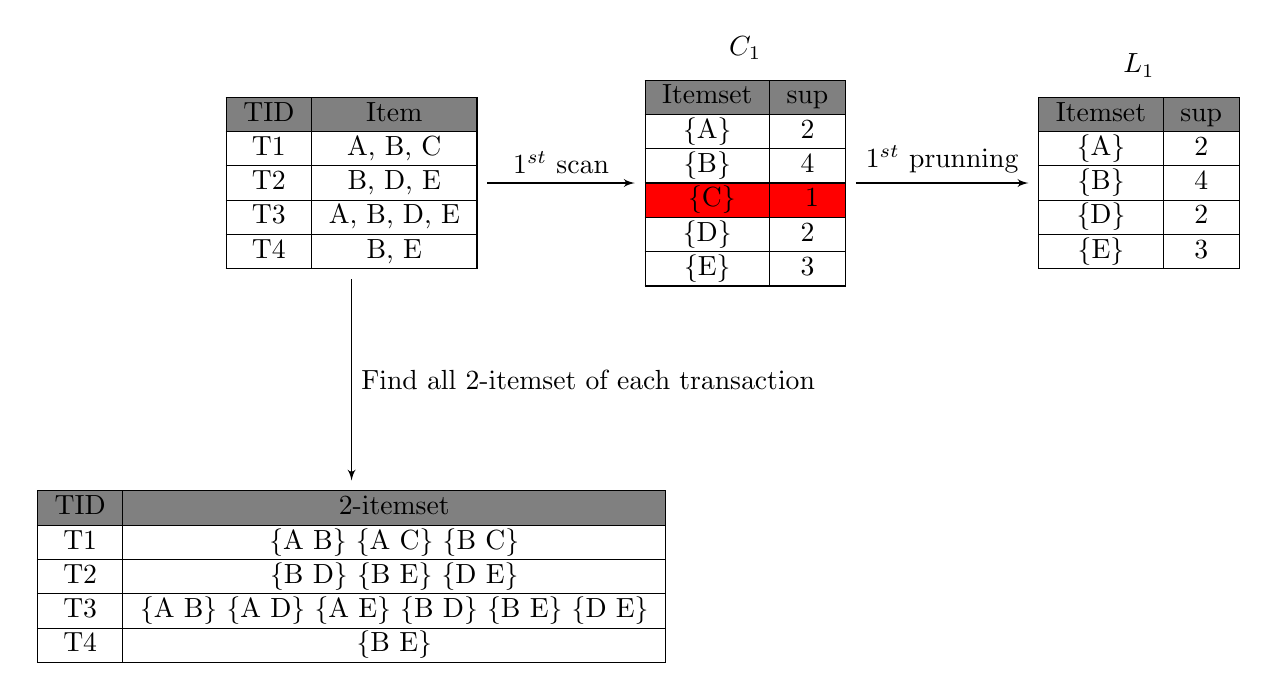
\begin{tikzpicture}[node distance = 5cm, auto]
  % Define block styles
  \tikzstyle{block} = [rectangle, fill=none,
                      text centered, rounded corners, minimum height=4em]
  \tikzstyle{line} = [draw, -latex']

  % Place nodes
  \node [block] (item1) {
    \begin{tabular}{|c|c|c|}
      \hline
        \rowcolor{Gray} % Set the color of the first row to gray
        TID & Item \\
        \hline
        T1 & A, B, C \\
        \hline
        T2 & B, D, E \\
        \hline
        T3 & A, B, D, E \\
        \hline
        T4 & B, E \\
        \hline
    \end{tabular}
  };

  \node [block, right of=item1, label=above:$C_1$] (scan1) {
    \begin{tabular}{|c|c|c|}
      \hline
        \rowcolor{Gray} % Set the color of the first row to gray
        Itemset & sup \\
        \hline
        {\{A\}} & 2 \\
        \hline
        {\{B\}} & 4 \\
        \hline
        \cellcolor{red} {\{C\}} & \cellcolor{red} 1 \\
        \hline
        {\{D\}} & 2 \\
        \hline
        {\{E\}} & 3 \\
        \hline
    \end{tabular}
  };

  \node [block, right of=scan1, label=above:$L_1$] (prunning1) {
    \begin{tabular}{|c|c|c|}
      \hline
        \rowcolor{Gray} % Set the color of the first row to gray
        Itemset & sup \\
        \hline
        {\{A\}} & 2 \\
        \hline
        {\{B\}} & 4 \\
        \hline
        {\{D\}} & 2 \\
        \hline
        {\{E\}} & 3 \\
        \hline
    \end{tabular}
  };

  \node [block, below of=item1] (2set) {
    \begin{tabular}{|c|c|c|}
      \hline
        \rowcolor{Gray} % Set the color of the first row to gray
        TID & 2-itemset \\
        \hline
        T1 & \{A B\} \{A C\} \{B C\} \\
        \hline
        T2 & \{B D\} \{B E\} \{D E\} \\
        \hline
        T3 & \{A B\} \{A D\} \{A E\} \{B D\} \{B E\} \{D E\} \\
        \hline
        T4 & \{B E\} \\
        \hline
    \end{tabular}
  };

  % Draw edges
  \path [line] (item1) -- (scan1) node[midway, above] {$1^{st}$ scan};
  \path [line] (scan1) -- (prunning1) node[midway, above] {$1^{st}$ prunning};
  \path [line] (item1) -- (2set) node[midway, right] {Find all 2-itemset of each transaction};

\end{tikzpicture}

Because we have:

\begin{itemize}
  \item Items = A, B, C, D, E,
  \item Order = 1, 2, 3, 4, 5
  \item Hash function : $h(\{x y\}) = (($order of $x)*10+($order of $y)) \% 7$
\end{itemize}

Thus we have the hash table below:

\begin{tabular}{|c|c|c|c|c|c|c|c|}
  \hline
    \rowcolor{Gray} % Set the color of the first row to gray
    bucket & 0 & 1 & 2 & 3 & 4 & 5 & 6 \\
    \hline
    count & 1 & 1 & 1 & 4 & 3 & 2 & 1 \\
    \hline
    2-itemset & \{A D\} & \{A E\} & \{B C\} & \{B D\} & \{B E\} & \{A B\} & \{A C\} \\
    &  &  &  & \{D E\} & \{B E\} & \{A B\} & \\
    &  &  &  & \{B D\} & \{B E\} &  &  \\
    &  &  &  & \{D E\} &  &  &  \\
    \hline
\end{tabular}

Let $L_1$*$L_1$ to generate a 2-itemset table, and choose the itemsets where the number of content in its bucket is above the minimum support.

\begin{tikzpicture}[node distance = 5.5cm, auto]
  % Define block styles
  \tikzstyle{block} = [rectangle, fill=none,
                      text centered, rounded corners, minimum height=4em]
  \tikzstyle{line} = [draw, -latex']

  % Place nodes
  \node [block] (2set) {
    \begin{tabular}{|c|c|c|}
      \hline
        \rowcolor{Gray} % Set the color of the first row to gray
        $L_1$*$L_1$ & \# in the bucket \\
        \hline
        \{A B\} & 2 \\
        \hline
        \cellcolor{red} \{A D\} & \cellcolor{red} 1 \\
        \hline
        \cellcolor{red} \{A E\} & \cellcolor{red} 1 \\
        \hline
        \{B D\} & 4 \\
        \hline
        \{B E\} & 3 \\
        \hline
        \{D E\} & 4 \\
        \hline
    \end{tabular}
  };

  \node [block, right of=item1, label=above:$C_2$] (C2) {
    \begin{tabular}{|c|}
      \hline
        \rowcolor{Gray} % Set the color of the first row to gray
        Resulted $C_2$ \\
        \hline
        \{A B\} \\
        \hline
        \{B D\} \\
        \hline
        \{B E\} \\
        \hline
        \{D E\} \\
        \hline
    \end{tabular}
  };

  \node [block, right of=C2, label=above:$L_2$] (L2) {
    \begin{tabular}{|c|c|}
      \hline
        \rowcolor{Gray} % Set the color of the first row to gray
        $C_2$ & sup \\
        \hline
        \{A B\} & 2 \\
        \hline
        \{B D\} & 2 \\
        \hline
        \{B E\} & 3 \\
        \hline
        \{D E\} & 2 \\
        \hline
    \end{tabular}
  };

  % Draw edges
  \path [line] (2set) -- (C2) node[midway, above] {};
  \path [line] (C2) -- (L2);
\end{tikzpicture}

Because if an item occurs in a frequent ($k$+1)-itemset,
it must occur in at least k candidate k-itemsets.

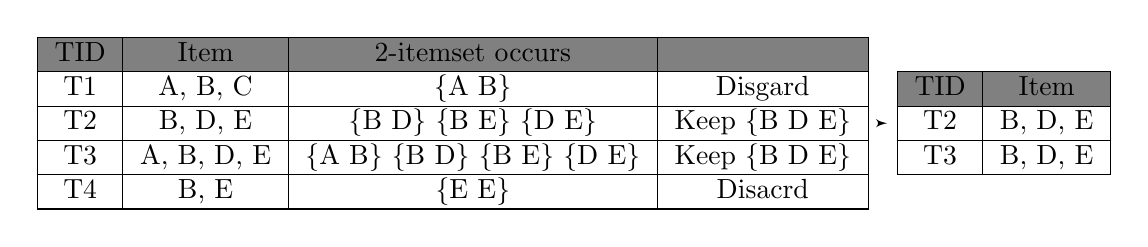
\begin{tikzpicture}[node distance = 7cm, auto]
  % Define block styles
  \tikzstyle{block} = [rectangle, fill=none,
                      text centered, rounded corners, minimum height=4em]
  \tikzstyle{line} = [draw, -latex']

  % Place nodes
  \node [block] (item1) {
    \begin{tabular}{|c|c|c|c|}
      \hline
      \rowcolor{Gray} % Set the color of the first row to gray
      TID & Item & 2-itemset occurs &  \\
      \hline
      T1 & A, B, C & \{A B\} & Disgard \\
      \hline
      T2 & B, D, E & \{B D\} \{B E\} \{D E\} & Keep \{B D E\} \\
      \hline
      T3 & A, B, D, E & \{A B\} \{B D\} \{B E\} \{D E\} & Keep \{B D E\}  \\
      \hline
      T4 & B, E & \{E E\} & Disacrd \\
      \hline
    \end{tabular}
  };

  \node [block, right of=item1] (item2) {
    \begin{tabular}{|c|c|c|}
      \hline
        \rowcolor{Gray} % Set the color of the first row to gray
        TID & Item \\
        \hline
        T2 & B, D, E \\
        \hline
        T3 & B, D, E \\
        \hline
    \end{tabular}
  };

  % Draw edges
  \path [line] (item1) -- (item2);
\end{tikzpicture}

Thus we have reduced the transactions.

\section*{Q3 [35 Marks]}

An itemset $X$ is said to be a frequent itemset if the frequency count of $X$ is at least a given support threshold.

An itemset $Y$ is a proper super-itemset of $X$ if $X \subset Y$ and $X \neq Y$. 

An itemset $X$ is said to be a closed frequent itemset 
if (1) $X$ is frequent 
and (2) there exists no proper super-itemset $Y$ of $X$ such that $Y$ is frequent 
and $Y$ has the same frequency count as $X$.

An itemset $X$ is said to be a maximal frequent itemset
if (1) $X$ is frequent
and (2) there exists no proper super-itemset $Y$ of $X$ such that $Y$ is frequent.

Let $F_c$ be the set of (traditional) frequent itemsets each of which is associated with a frequency in the dataset.

For example, if there are three frequent itemsets, \{$I_1$\} with frequency 4,
\{$I_2$\} with frequency 5, and \{$I_1, I_2$\} with frequency 3,
$F$=\{\{$I_1$\}, \{$I_2$\}, \{$I_2, I_2$\}\}
and $F_c = \{<\{I_1\}, 4>, <\{I_2\}, 5>, <\{I_1, I_2\}, 3>\}$.

Similarly, let $C$ be the set of closed frequent itemsets without specifying the frequency of itemsets.

Let $C_c$ be the set of closed frequent itemsets each of which is associated with a frequency of itemsets.

Let $M$ be the set of maximal frequent itemsets without specifying the frequency of itemsets.

Ler $M_c$ be the set of maximal frequent itemsets each of which is associated with a frequency in the dataset.

The following shows six transactions with four items.
Each row corresponds to a transaction where 1 corresponds to a presence of an item and 0 corresponds to an absence.

\begin{tabular}{|c|c|c|c|}
  \hline
    \rowcolor{Gray} % Set the color of the first row to gray
    A & B & C & D \\
    \hline
    0 & 0 & 1 & 1 \\
    \hline
    1 & 1 & 0 & 0 \\
    \hline
    0 & 0 & 1 & 1 \\
    \hline
    1 & 0 & 1 & 1 \\
    \hline
    1 & 0 & 0 & 0 \\
    \hline
    0 & 0 & 0 & 1 \\
    \hline
\end{tabular}

Suppose that the support threshold is 2.

(a) (i) What is $F_C$? \hspace{1cm} (ii) What is $C_c$? \hspace{1cm} (iii)What is $M_c$? \textbf{(5 Marks)}

(b) (i) What is the advantages and the disadvantages of using closed frequent itemsets compared with traditional frequent itemsets? \textbf{(5 Marks)}

(ii) What are the advantages and the disadvantages of using closed frequent itemsets compared with maximal frequent itemsets? \textbf{(5 Marks)}

(c) Please adapt algorithm FP-growth with the use of the FP-tree to find all closed frequent item set.
Please write down how to adapt algorithm FP-growth and illustrate the adapted algorithm with the above example. \textbf{(20 Marks)}

\subsection*{Solution}

\paragraph*{(a)} According to the topic, we have the following transaction database. And we generate all the $k$-itemsets which might be frequent itemsets.

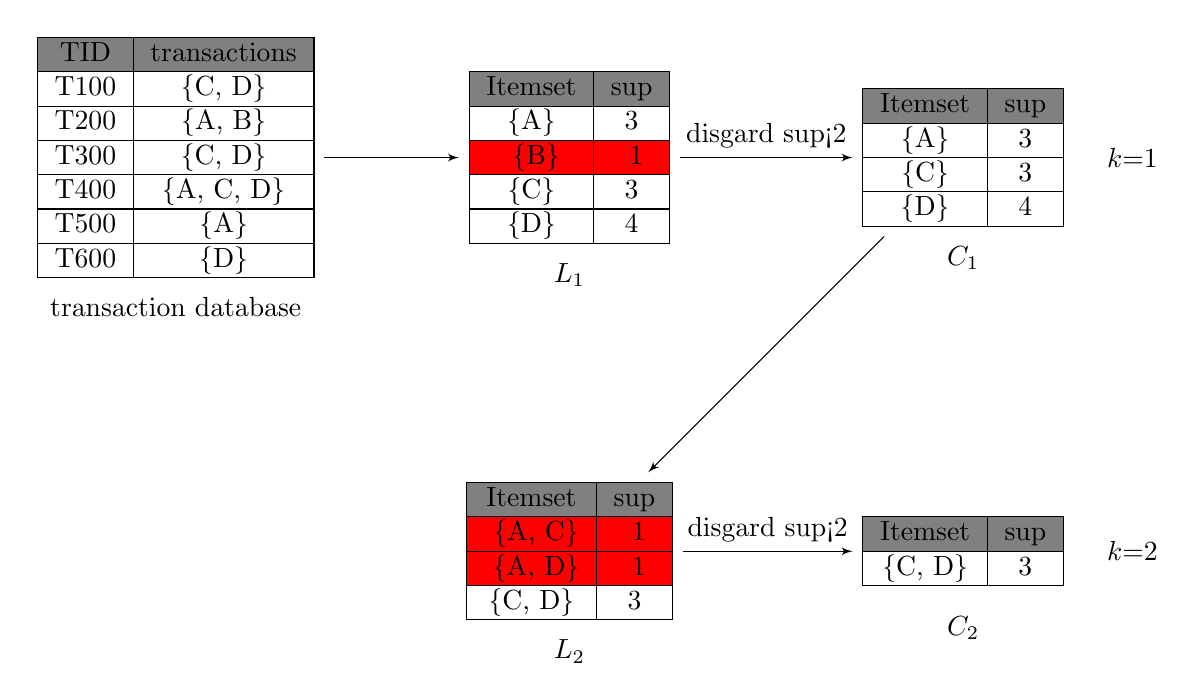
\begin{tikzpicture}[node distance = 5cm, auto]
  % Define block styles
  \tikzstyle{block} = [rectangle, fill=none,
                      text centered, rounded corners, minimum height=4em]
  \tikzstyle{line} = [draw, -latex']

  % Place nodes
  \node [block, label=below:{transaction database}] (DB) {
    \begin{tabular}{|c|c|}
      \hline
        \rowcolor{Gray} % Set the color of the first row to gray
        TID & transactions \\
        \hline
        T100 & \{C, D\} \\
        \hline
        T200 & \{A, B\} \\
        \hline
        T300 & \{C, D\} \\
        \hline
        T400 & \{A, C, D\} \\
        \hline
        T500 & \{A\} \\
        \hline
        T600 & \{D\} \\
        \hline
    \end{tabular}
  };

  \node [block, right of=DB, label=below:{$L_1$}] (L1) {
    \begin{tabular}{|c|c|}
      \hline
      \rowcolor{Gray} % Set the color of the first row to gray
      Itemset & sup  \\
      \hline
      \{A\} & 3 \\
      \hline
      \cellcolor{red} \{B\} & \cellcolor{red} 1 \\
      \hline
      \{C\} & 3  \\
      \hline
      \{D\} & 4 \\
      \hline
    \end{tabular}
  };

  \node [block, right of=L1, label=below:{$C_1$}] (C1) {
    \begin{tabular}{|c|c|}
      \hline
        \rowcolor{Gray} % Set the color of the first row to gray
        Itemset & sup \\
        \hline
        \{A\} & 3 \\
        \hline
        \{C\} & 3 \\
        \hline
        \{D\} & 4 \\
        \hline
    \end{tabular}
  };

  \node[left=of C1, xshift = 9cm] {$k$=1};

  \node [block, below of=L1, label=below:{$L_2$}] (L2) {
    \begin{tabular}{|c|c|}
      \hline
        \rowcolor{Gray} % Set the color of the first row to gray
        Itemset & sup \\
        \hline
        \cellcolor{red} \{A, C\} & \cellcolor{red} 1 \\
        \hline
        \cellcolor{red} \{A, D\} & \cellcolor{red} 1 \\
        \hline
        \{C, D\} & 3 \\
        \hline
    \end{tabular}
  };

  \node [block, right of=L2, label=below:{$C_2$}] (C2) {
    \begin{tabular}{|c|c|}
      \hline
        \rowcolor{Gray} % Set the color of the first row to gray
        Itemset & sup \\
        \hline
        \{C, D\} & 3 \\
        \hline
    \end{tabular}
  };

  \node[left=of C2, xshift = 9cm] {$k$=2};

  % Draw edges
  \path [line] (DB) -- (L1);
  \path [line] (L1) -- (C1) node [midway, above] {disgard sup<2};
  \path [line] (C1) -- (L2) node [midway, above] {};
  \path [line] (L2) -- (C2) node [midway, above] {disgard sup<2};
\end{tikzpicture}

\textbf{i}: We have $F_c = \{ <\{A\},3>, <\{C\},3>, <\{D\},4>, <\{C, D\},3>\}$

\textbf{ii}: We have $C_c = \{ <\{A\},3>, <\{C, D\},3>\}$

\textbf{iii}: We have $M_c = \{ <\{A\},3>, <\{C, D\},3>\}$

\paragraph*{(b)}

\paragraph*{(c)}

\section*{Q4 [35 Marks]}

A GSP example: Suppose now we have 5 events: 'Upload Songs', 'Add Tags', 'Share', 'Listen' and 'Comment'.
Let min-support be 40\%.
The sequence database of a Music Platform is shown in following table:

\begin{tabular}{|c|c|}
  \hline
    \rowcolor{Gray} % Set the color of the first row to gray
    Object & Sequence \\
    \hline
    A & <\{'Upload Songs', 'Add Tags'\}> \\
    \hline
    B & <\{'Upload Songs', 'Share'\}> \\
    \hline
    C & <\{'Upload Songs'\}, \{'Share', 'Listen'\}> \\
    \hline
    D & <\{'Upload Songs'\}, \{'Upload Songs', 'Add Tags'\}, \{'Listen'\}> \\
    \hline
    E & <\{'Listen'\}, \{'Add Tags', 'Comment'\}, \{'Share', 'Listen'\}> \\
    \hline
\end{tabular}

Please answer the following questions:

(a) Make the first pass over the sequence database to yield all the 1-element \textbf{frequent} sequences and What is the corresponding support? \textbf{5 Marks}

(b) Based on (a), do the 2-sequences Candidate Generation and Candidate Pruning. \textbf{10 Marks}

(c) What is the \textbf{frequent} 2-sequences based on the result of (b)? \textbf{5 Marks}

(d) Based on (c), do the 3-sequences Candidate Generation and Candidate Pruning.
When a sequence should be pruned, you need to explain why. \textbf{10 Marks}

(e) What is the frequent 3-sequences based on the result of (d)?
Please calculate the support. \textbf{5 Marks}

\textbf{Remember: For frequent k-sequences, the support >= min-support}

\subsection*{Solution}

\end{document}
